\documentclass{article}
\usepackage{graphicx}
\usepackage{fancyhdr}
\usepackage{xcolor}
\usepackage{listings}
\usepackage{graphicx}
\usepackage{subcaption} % Package for subfigures
\usepackage{caption}
\usepackage{placeins}
\usepackage{media9}

\usepackage{amsmath} % Package for mathematical equations
% Define custom commands
\usepackage{listings} % Package for including code snippets
\usepackage{xcolor} % Package for coloring text
\newcommand{\thetitle}{Robotics Assignment}
\newcommand{\thecoursecode}{2MEOE51}
\newcommand{\thecoursename}{Robotics}
\newcommand{\therollnumbers}{21bce201, 21bce203, 21bce320, 21bce187,21bce216,21bce224}
\newcommand{\thelogo}{logo.png} % Update with your logo file path

% Page headers
\pagestyle{fancy}
\fancyhf{}
\rhead{\thetitle}
\lhead{\thecoursecode}
\rfoot{\thepage}
\lstdefinestyle{ArduinoStyle}{
    language=C++, % Set the language
    basicstyle=\small\ttfamily, % Basic font style and size
    keywordstyle=\color{blue}, % Keywords style
    commentstyle=\color{green!40!black}, % Comments style
    stringstyle=\color{red}, % Strings style
    numbers=left, % Line numbers on the left
    numberstyle=\tiny, % Line numbers font size
    stepnumber=1, % Line numbers incrementing
    numbersep=5pt, % Distance from line numbers to code
    frame=single, % Single frame around code
    breaklines=true, % Enable line breaking
    tabsize=2, % Tab size
    captionpos=b, % Position of the caption
    xleftmargin=15pt, % Left margin
    framexleftmargin=15pt, % Extra left margin from frame
}

% Define settings for including MATLAB code
\lstset{
    language=Matlab,
    basicstyle=\small\ttfamily,
    keywordstyle=\color{blue},
    commentstyle=\color{green!40!black},
    stringstyle=\color{red},
    showstringspaces=false,
    numbers=left,
    numberstyle=\tiny,
    stepnumber=1,
    numbersep=5pt,
    frame=single,
    breaklines=true,
    tabsize=2,
    captionpos=b,
    xleftmargin=15pt,
    framexleftmargin=15pt,
    morekeywords={drawCircle, drawEllipse, drawPolygon, inverseKinematics, plotArm}
}

\begin{document}

% Cover Page
\begin{titlepage}
    \centering
    \vspace*{2cm}
    {\LARGE \thecoursename \par}
    \vspace{1.5cm}
    \includegraphics[width=0.5\textwidth]{image.png} % Include the logo
    \par\vspace{1cm}
    {\huge\bfseries \thetitle \par}
    \vspace{1cm}
    {\Large \therollnumbers \par}
    \vfill
    {\large \textsc{IT, NU}\par}
    \vspace{0.5cm}
    {\large \today\par}
\end{titlepage}

% Table of Contents
\tableofcontents
\newpage

% Problem Statement and Objectives
\section{Problem Statement and Objectives}
Develop a 2 DOF planar robotic arm capable of drawing various 2D geometries, including circles, ellipses, and polygons based on user input. The robot should accept input data such as circle radius, ellipse major and minor axes lengths, or polygon vertices coordinates and accurately draw the specified geometry.

% Design Specifications
\section{Design Specifications}
\begin{itemize}
    \item Two degrees of freedom for planar movement (e.g., base rotation and elbow joint)
    \item Precise end-effector positioning for drawing
    \item Interface for receiving user input and translating it into robotic arm motion
\end{itemize}

% Implementation Details
\section{Implementation Details}
\begin{itemize}
    \item Selection of appropriate actuators (e.g., servo motors) for joint control
    \item Kinematic analysis for forward and inverse kinematics calculations
    \item Integration of microcontroller (e.g., Arduino) for actuator control and user input handling
    \item Programming control algorithms to map geometry parameters to robotic arm commands
\end{itemize}

% Forward and Inverse Kinematics
% \section{Forward and Inverse Kinematics}
% Forward kinematics refers to the mathematical calculations that determine the position and orientation of the end-effector (drawing tool) based on the joint angles of the robotic arm. Inverse kinematics involves calculating the joint angles required to position the end-effector at a desired location in the workspace.
\section{Forward Kinematics}
Forward kinematics refers to the mathematical calculations that determine the position and orientation of the end-effector (drawing tool) based on the joint angles of the robotic arm.
Forward kinematics is used to determine the position of the end-effector (tip of the robotic arm) based on the joint angles \( \theta_1 \) and \( \theta_2 \).

Given:
\begin{itemize}
    \item Length of link 1 (shoulder to elbow): \( L_1 \)
    \item Length of link 2 (elbow to end-effector): \( L_2 \)
    \item Joint angles:
    \begin{itemize}
        \item \( \theta_1 \): Angle of the first joint (shoulder)
        \item \( \theta_2 \): Angle of the second joint (elbow)
    \end{itemize}
\end{itemize}

The forward kinematics equations are:
\begin{align*}
x &= L_1 \cos(\theta_1) + L_2 \cos(\theta_1 + \theta_2) \\
y &= L_1 \sin(\theta_1) + L_2 \sin(\theta_1 + \theta_2)
\end{align*}
where \( (x, y) \) are the Cartesian coordinates of the end-effector.

\section{Inverse Kinematics}
Inverse kinematics involves calculating the joint angles required to position the end-effector at a desired location in the workspace.
Inverse kinematics is used to calculate the joint angles \( \theta_1 \) and \( \theta_2 \) required to position the end-effector at a desired point \( (x, y) \).

Given:
\begin{itemize}
    \item Desired coordinates of the end-effector: \( (x, y) \)
    \item Length of link 1 (shoulder to elbow): \( L_1 \)
    \item Length of link 2 (elbow to end-effector): \( L_2 \)
\end{itemize}

The inverse kinematics equations are:
\begin{align*}
c_2 &= \frac{x^2 + y^2 - L_1^2 - L_2^2}{2 \times L_1 \times L_2} \\
s_2 &= \pm \sqrt{1 - c_2^2} \quad \text{(Choose appropriate sign based on constraints)} \\
\theta_2 &= \text{atan2}(s_2, c_2) \\
\theta_1 &= \text{atan2}(y, x) - \text{atan2}(L_2 \times s_2, L_1 + L_2 \times c_2)
\end{align*}
where \( c_2 \) and \( s_2 \) are the cosine and sine values of \( \theta_2 \), respectively.

These equations will allow you to calculate the joint angles required to position the end-effector of your 2-DOF robotic arm at a desired location \( (x, y) \).


% MATLAB Code
\section{MATLAB Code for Geometry Generation}
\lstinputlisting[caption={MATLAB Code for 2 DOF Planar Robotic Arm}, label=lst:matlab]{code.m}

% Output Images
\section{Output Images}

\begin{figure*}[]
    

    \centering
    \begin{subfigure}[b]{0.8\textwidth}
        \centering
        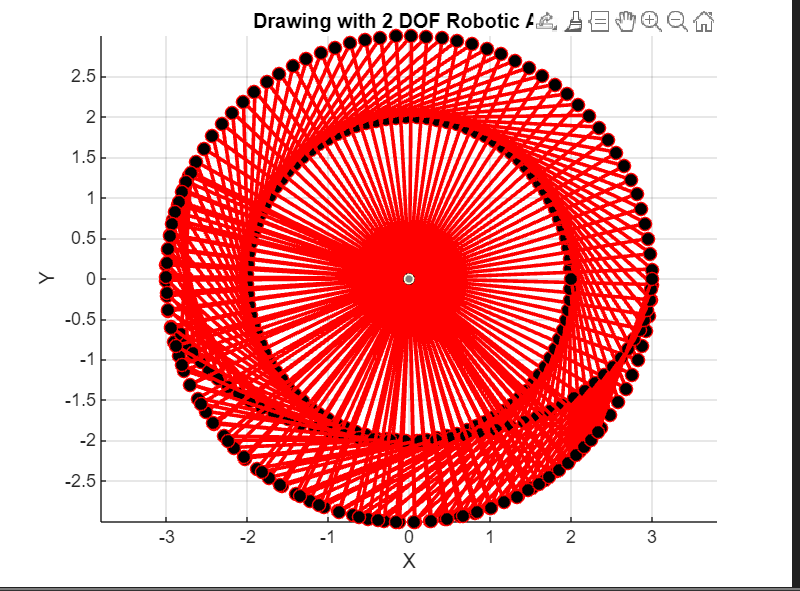
\includegraphics[width=\textwidth]{image_1.png}
        \caption{Output 1: Circle}
        \label{fig:output-circle}
    \end{subfigure}
    \\
    \begin{subfigure}[b]{0.8\textwidth}
        \centering
        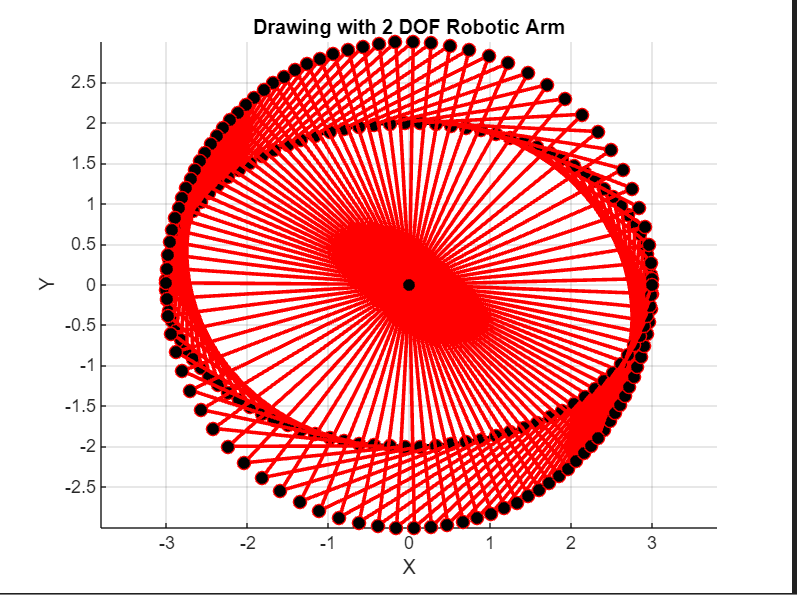
\includegraphics[width=\textwidth]{image_2.png}
        \caption{Output 2: Ellipse}
        \label{fig:output-ellipse}
    \end{subfigure}
    \\
    \begin{subfigure}[b]{0.8\textwidth}
        \centering
        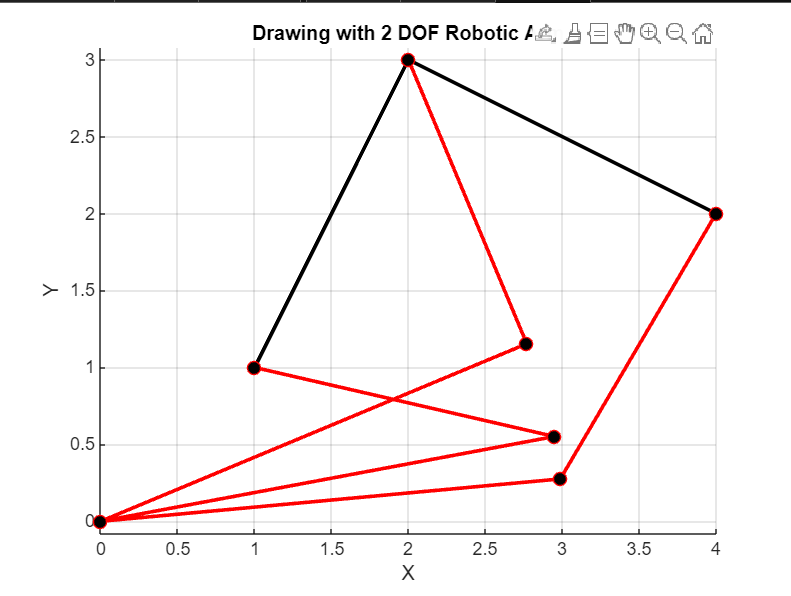
\includegraphics[width=\textwidth]{imag_3.png}
        \caption{Output 3: Polygon}
        \label{fig:output-polygon}
    \end{subfigure}
    \caption{Output Images}
    \label{fig:output-images}
\end{figure*}

% TinkerCAD Wiring Diagram
% \section{TinkerCAD Wiring Diagram}
% \begin{figure}[htbp]
%     \centering
%     \caption{TinkerCAD Wiring Diagram of Servo Motors}
%     % \includegraphics[width=0.8\textwidth]{tinkercad-diagram.png}
%     \label{fig:tinkercad}
% \end{figure}

% Arduino Program
% \section{Arduino Program}




\section{Arduino Program for Robotic Arm Control}

Below is the Arduino program to control a 2-DOF robotic arm using servo motors based on joint angles received via serial communication.

\begin{lstlisting}[style=ArduinoStyle, caption={Arduino Program for Robotic Arm Control}, label=arduino]
#include <Servo.h>

// Define servo motor pins
const int servoPin1 = 9;  // Pin for servo motor controlling joint 1
const int servoPin2 = 10; // Pin for servo motor controlling joint 2

// Create servo objects
Servo servo1;
Servo servo2;

void setup() {
  // Attach servos to their respective pins
  servo1.attach(servoPin1);
  servo2.attach(servoPin2);
}

void loop() {
  // Read joint angles from serial input
  if (Serial.available() >= 2 * sizeof(float)) {
    float theta1, theta2;
    
    // Read theta1 (shoulder angle)
    theta1 = Serial.parseFloat();
    
    // Read theta2 (elbow angle)
    theta2 = Serial.parseFloat();

    // Map joint angles to servo motor positions (0-180 degrees)
    int servoPos1 = map(theta1, -PI, PI, 0, 180);
    int servoPos2 = map(theta2, -PI, PI, 0, 180);

    // Move servo motors to the calculated positions
    servo1.write(servoPos1);
    servo2.write(servoPos2);

    // Delay to allow servos to reach the desired positions
    delay(100);
  }
}
\end{lstlisting}

\section{Instructions for Use}

\begin{enumerate}
  \item **Servo Configuration**:
     - Connect two servo motors to Arduino, one for each joint of the robotic arm (`servoPin1` for joint 1 and `servoPin2` for joint 2).
  
  \item **Arduino Setup**:
     - Install the `Servo` library in your Arduino IDE if not already installed.
     - Upload the above Arduino sketch to your Arduino board.
  
  \item **Communicating with Arduino**:
     - Send joint angles (`theta1` and `theta2`) from your MATLAB or other control program to Arduino via serial communication.
     - Ensure that the angles are sent as floats separated by spaces (e.g., `"1.57 2.09"`).
  
  \item **Mapping Angles to Servo Positions**:
     - Use `map()` function to convert the calculated joint angles (`-PI` to `PI` radians) into servo positions (`0` to `180` degrees).
  
  \item **Controlling Servo Motors**:
     - Use `servo1.write()` and `servo2.write()` to set the servo positions based on the mapped values of `theta1` and `theta2`.
  
  \item **Adjust Delay**:
     - Adjust the delay time (`delay(100)`) as needed to allow the servo motors to reach the desired positions smoothly.
\end{enumerate}

By running this Arduino program, you can control the robotic arm's joint angles in real-time based on the input from your MATLAB code (or any other control source) via serial communication. Ensure that the serial baud rate and communication protocol match between MATLAB and Arduino for reliable data transmission.

% Images of Actual Robot
\section{Images of Actual Robot}
\FloatBarrier

\begin{figure}[h!]
    \centering
     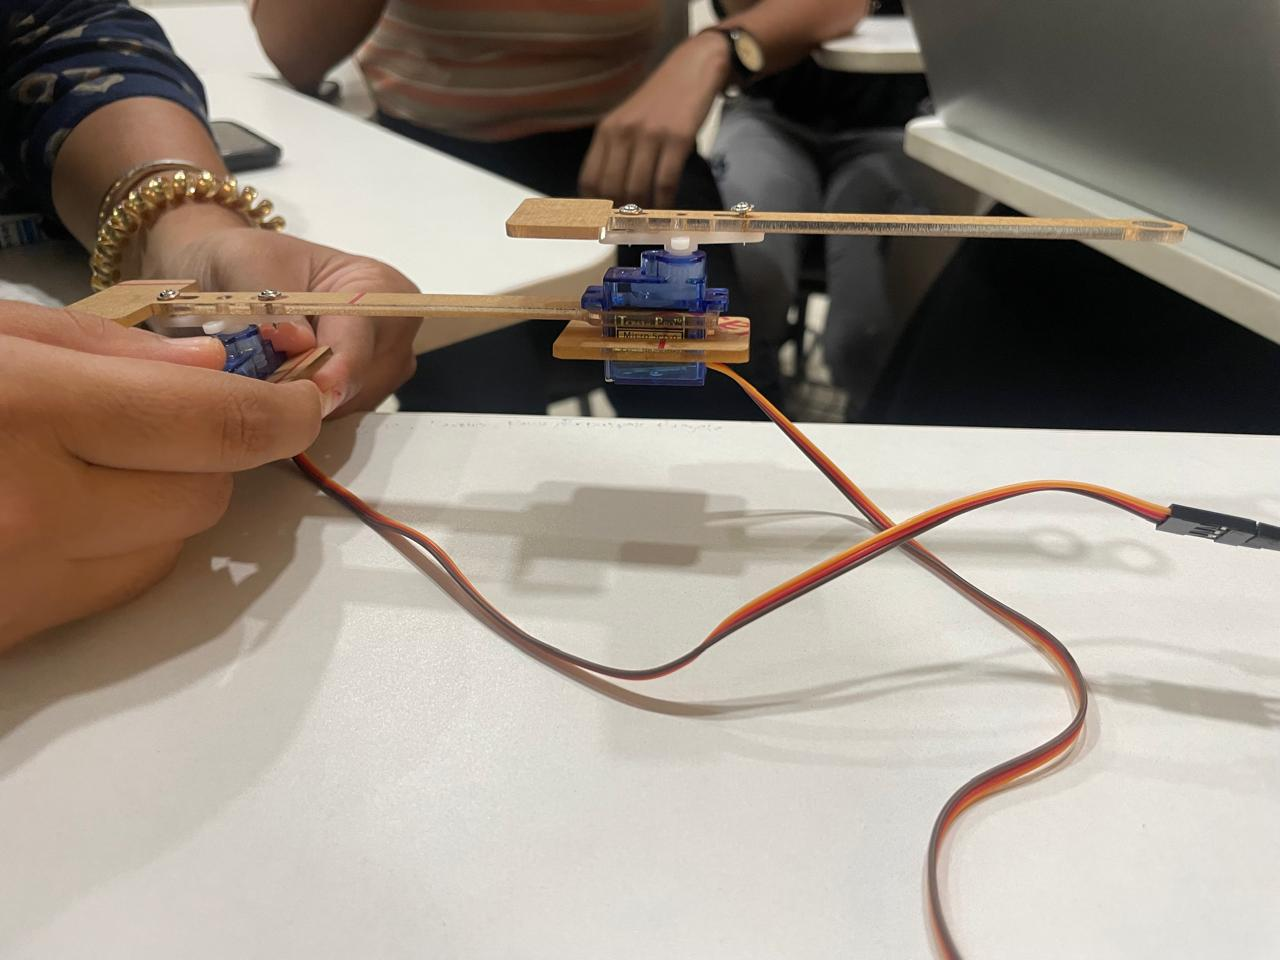
\includegraphics[width=1\textwidth]{robo_arm.jpg}
    \caption{Images of the Actual Robot}
    \label{fig:robot-images}
\end{figure}

% Working Video
\section{Working Video}




\end{document}
